%=======================================================================
% CVS: $Id: ice_refdoc.tex 5 2005-12-12 17:41:05Z mvr $
% CVS: $Source$
% CVS: $Name$
%=======================================================================

\documentclass[]{article}
\usepackage{html}
\usepackage{natbib}
%\usepackage{supertabular}
\setcounter{tocdepth}{7}
\setcounter{secnumdepth}{10}

% create conditional that senses pdf output
\newif\ifpdf
\ifx\pdfoutput\undefined
   \pdffalse
\else
   \pdfoutput=1
   \pdftrue
\fi

% supply correct option to graphicx
\ifpdf
   \usepackage[pdftex]{graphicx}
   \pdfcompresslevel=9
\else
   \usepackage{graphicx}
\fi

\textheight=9.0in
\textwidth=6.5in
\evensidemargin=0.0in
\oddsidemargin=0.0in
\footskip=0.4in   % Positions page number 1 in is too big%
\topmargin=0.0in
\headheight=0.0in
\headsep = 0.0in

\begin{document}
\bodytext{BGCOLOR=white LINK=#083194 VLINK=#21004A}

% This is a modified definition of Ventry from The Latex Companion, p. 64
 \newenvironment{Ventry}[1]%
   {\begin{list}{}{\renewcommand{\makelabel}[1]{\textsf{##1:}\hfil}%
      \settowidth{\labelwidth}{\textsf{#1:}}%
      \setlength{\leftmargin}{1.5cm}%
      \setlength{\labelwidth}{1.0cm}%
      \setlength{\itemsep}{0pt}%
      \setlength{\parsep}{0pt}}}%
   {\end{list}}


% supply correct file suffix to graphicx
\ifpdf
\DeclareGraphicsExtensions{.jpg,.pdf}
\else
\DeclareGraphicsExtensions{.eps,.ps}
\fi

\begin{titlepage}

\vspace*{2in}

\begin{center}
{\Large
  {\bf Community Sea Ice Model (CSIM) Developer's Guide} \\
  {\bf Code Reference for Version 5.0} \\
  \vspace{0.2in}
  {Released with CCSM3.0} \\
  \vspace{.5in}
  Julie Schramm \\
  Cecilia Bitz  \\
  Bruce Briegleb \\
  Marika Holland \\
  Elizabeth Hunke \\
  Bill Lipscomb \\
  Dick Moritz \\
}
\end{center}

\vspace{2in}
\begin{tabular}{p{5in}p{.9in}}
\noindent {\bf Community Climate System Model} \\
\noindent National Center for Atmospheric Research, Boulder, CO \\
\noindent http://www.cgd.ucar.edu/csm/models \\
\hline
\noindent CVS tag \verb+ $Name$  +  Build date: \today \\
\end{tabular}

\end{titlepage}

%===============================================================================

\tableofcontents

\newpage
%===============================================================================


\section {Overview}

This code reference guide accompanies the CSIM5 User's Guide, and is intended
for those whose research requires modifications to the source code rather than 
to the scripts or the namelists.  It is also meant to provide guidance
to users developing code for incorporation into CSIM.  This is only the second
version of this document, so it contains limited information, including a CSIM5
calling tree, some information on the technical aspects of the code, and the
code-interface information generated by the ProTeX utility.  It also includes the
CSIM coding standard and a procedure for integrating software into CSIM.

CSIM is typically run coupled in which case it receives forcing information from
other model components via a flux coupler.  It has been developed to run as the
sea ice component of the NCAR CCSM (Community Climate System Model).  When running uncoupled,
CSIM reads in forcing data from a set of files. Both configurations use the
same source code, so this document can be used with both applications.

The CSIM source code is based on the Los Alamos sea ice model, CICE.
After a code merger with CICE was carried out to take advantage of the vector-
friendly code, the models are very similar.  If there are some topics that
are not covered in the CSIM documentation, users are encouraged to look
at the CICE documentation \cite[]{cice04}.  It is available at
http://climate.lanl.gov/Models/CICE/index.htm.

An attempt has been made throughout this document to provide the following
text convention.  Variable names used in the code are {\tt typewritten}.
Subroutine names are given in {\it italic}, and file names are in {\bf boldface}.
Hereafter, terms shown in {\bf \textsl{slanted boldface}} the first time they
appear in the text are defined in the Glossary. 

%=======================================================================

\subsection {CCSM Directory Structure}
\label{sec:ccsm_dir_structure}

{\bf \textsl{CSIM5}} is located under the {\bf \textsl{CCSM}} models and ice subdirectories.
The directory structure of CSIM5 within CCSM is shown below.  The root directory name of CSIM
remains as {\bf csim4} due to the difficulty of changing it in the source code repository.

\begin{verbatim}
                                ccsm3         (main directory) 
                                  |
                                  |
                 models-----------+------------ scripts
                    |                              |
                    |                              |
      bld--------csm_share-------ice           (build scripts for
       |            |             |             coupled model)
   (Makefile  (share code         |               
    macros)    subdirectory)      | 
                                csim4         (active ice component)
                                  |
                      docs -------+------- src 
                       |                    | 
                     (CSIM                  |
                  documentation)            |
                                            |
                                            |
       bld ------------ input_templates ----+---- source ------ build scripts
       |                    |                       |           for uncoupled
  (Makefile macros     (resolution-dependent    (F90 source     ice model
   for uncoupled         input files)              code) 
    ice model)
\end{verbatim}

Only the branches referenced in this document appear in the Figure. There
are separate directories for the build scripts and the {\bf Macros.*} files for
the coupled model and the uncoupled ice model. The {\bf Macros.*} files
contain machine dependent information for building the model.  The coupled
model uses the {\bf Macros.*} files in {\bf ccsm3/models/bld}, and the
uncoupled ice model uses those in {\bf ccsm3/models/ice/csim4/src/bld}.
To make modifications to the coupled model setup, modify the scripts in 
{\bf ccsm3/scripts}.  The setup scripts for the uncoupled model are
located in {\bf ccsm3/models/ice/csim4/src}.  The files located under
the main ice model directory {\bf /csim4/src} are described in the next section.

%\subsection {CSIM Directory Structure}
%=======================================================================
% CVS: $Id: ice_module_desc.tex 5 2005-12-12 17:41:05Z mvr $
% CVS: $Source$
% CVS: $Name$
%=======================================================================

\subsection {CSIM Module Descriptions}
\label{sec:csim_dir_structure}

The ice model uses {\bf \textsl{ProTex}}, which is a tool for self-documenting source code.
ProTex is a perl script that produces a LaTeX compatible document from 
Fortran source code that contains a ProTex prologue at the top of each module,
function and subroutine. The output from ProTex can be over 100 pages, and
make files and build scripts would not be included in any documentation
created by the ProTex tool.  In light of this, the ice model source code and
the build scripts are described briefly in this section.  There is additional
information in the code at the top of each module, subroutine and function. 

\begin{description}
  \item [csim4/src/csim.setup.csh] compiles the uncoupled ice model and prestages
                             the input data, contains the namelist, used
                             by {\bf csim\_run}
  \item [csim4/src/csim\_run] runs the uncoupled ice model
  \item [csim4/src/IBM\_tests] runs debug and exact restart tests on the {\bf \textsl{NCAR}}
                  IBM for the uncoupled ice model
  \item [csim4/src/bld/Macros.OS] macro definitions for supported operating systems, 
                            used by {\bf Makefile}
  \item [csim4/src/bld/makdep.c] perl script that determines module dependencies
  \item [csim4/src/bld/Makefile] builds the uncoupled ice model
  \item [csim4/src/input\_templates/ice\_model\_size.F.*] input files prestaged by 
                               {\bf csim.setup.csh} depending on the grid dimensions
                               and number of ice thickness categories set in this file.
\end{description}

Below is a list of one-line descriptions for the ice model modules from {\bf csim4/src/source}.

\begin{description}
  \item [ice.F]                     main program 
  \item [ice\_albedo.F]             albedo parameterization
  \item [ice\_atmo.F]               stability-based parameterization for calculating
                                        turbulent ice-atmosphere fluxes
  \item [ice\_calendar.F]           time manager
  \item [ice\_constants.F]          parameters, physical and numerical constants
  \item [ice\_coupling.F]           interface with flux coupler
  \item [ice\_diagnostics.F]        diagnostic and debugging routines
  \item [ice\_domain.F]             {\bf \textsl{MPI}} subdomain sizes and parallel processing info
  \item [ice\_dyn\_evp.F]           elastic-viscous-plastic dynamics component
  \item [ice\_exit.F]               aborts the model and prints error message
  \item [ice\_fileunits.F]          unit numbers for I/O
  \item [ice\_flux.F]               fluxes needed/produced by the model
  \item [ice\_flux\_in.F]           routines to read and interpolate forcing for stand-alone ice model
  \item [ice\_grid.F]               grids and land masks
  \item [ice\_history.F]            netCDF output routines and read/write restart
  \item [ice\_init.F]               namelist and initializations
  \item [ice\_itd.F]                utilities for managing ice thickness distribution
  \item [ice\_itd\_linear.F]        linear remapping for transport in thickness space
  \item [ice\_kinds\_mod.F]         definitions of reals, integers, etc.
  \item [ice\_mechred.F]            mechanical redistribution (ridging)
  \item [ice\_model\_size.F]        grid size, number of thickness categories and vertical layers
  \item [ice\_mpi\_internal.F]      utilities for internal MPI parallelization
  \item [ice\_ocean.F]              slab ocean mixed layer model
  \item [ice\_prescribed.F]         prescribed ice (not supported in this release)
  \item [ice\_read\_write.F]        utilities for reading/writing files
  \item [ice\_scaling.F]            ice-area scaling of fluxes sent to coupler
  \item [ice\_state.F]              arrays defining ice state 
  \item [ice\_therm\_itd.F]         thermodynamics changes mostly due to ITD (post-coupling)
  \item [ice\_therm\_vertical.F]    vertical growth rates and fluxes (pre-coupling thermodynamics)
  \item [ice\_timers.F]             timing routines 
  \item [ice\_transport\_mpdata.F]  horizontal advection via MPDATA or upwind
  \item [ice\_transport\_remap.F]   horizontal advection via incremental remapping
  \item [ice\_work.F]               globally accessible work arrays
\end{description}


%\subsection {External Software and Libraries}
%=======================================================================
% CVS: $Id: ice_softw_libs.tex 5 2005-12-12 17:41:05Z mvr $
% CVS: $Source$
% CVS: $Name$
%=======================================================================

\subsection {External Software and Libraries}

The CSIM code includes references to subroutines and libraries not contained in 
{\bf models/ice/csim4}.  This code is described in the following sections.

\subsubsection {CCSM Share Code}

CSIM uses some of the CCSM shared-code modules that are included in the
{\bf models/csm\_share} directory.  The share-code modules presently used in
CSIM are:

  \begin{itemize}
    \item {\bf shr\_const\_mod.F90} - This module contains the "shared constants"
          that are used by all components for CCSM.  Note that these constants
          are not used for the uncoupled ice model, which uses those set in
          {\bf ice\_constants.F}.

    \item {\bf shr\_kind\_mod.F90} - This module defines variable precision
          used by other shared-code modules.

    \item {\bf shr\_msg\_mod.F90} - This contains subroutines that provide an
          architecture-independent means of interacting with the operating system. CSIM
          uses the following subroutines from this module:

      \begin{itemize}
        \item {\it shr\_msg\_chdir} - changes current working directory
        \item {\it shr\_msg\_dirio} - redirects standard input and output to
                                    named files
      \end{itemize}

    \item {\bf shr\_mpi\_mod.F90} -  used by {\bf shr\_sys\_mod.F90}

    \item {\bf shr\_sys\_mod.F90} - This contains subroutines that provide an
          architecture-independent means of interacting with the operating system. CSIM
          uses the following routines from this module:
      \begin{itemize}
          \item {\it shr\_sys\_flush} - clears the print buffer
          \item {\it shr\_sys\_abort} - provides a consistent stopping mechanism for
                                      multiple processors
      \end{itemize}
  \end{itemize}

\subsubsection {netCDF Library}

The netCDF library is necessary to run CSIM.  The slab ocean mixed layer model and
the prescribed ice model (not supported in this release) read in forcing data from
netCDF files. The output history files are also written in this format. The history
files conform to the NetCDF Climate and Forecast (CF) Metadata Conventions 
(http://www.cgd.ucar.edu/cms/eaton/cf-metadata/index.html).
All of the netCDF-specific code used to write the history files is in subroutine
{\it icecdf} in module {\bf ice\_history.F}.   Machine dependent information that
sets the location of the netCDF library is set in the {\bf models/bld/Macros.*}
for the coupled model, and in {\bf models/ice/csim4/src/bld/Macros.*} for the
uncoupled ice model.


\subsubsection {Message Passing Interface (MPI)}

CSIM intra- and inter-model communications are conducted via MPI. The MPI
library is automatically loaded during the CCSM build procedures.



%=======================================================================
\section {Model Structure}

CSIM5 is written in the Fortran 90 programming language in fixed source
form.   It is parallelized internally by grid decomposition using
{\bf \textsl{MPI}} (Message Passing Interface).  There is an external layer of
parallelization, also using MPI, that allows message passing between the ice
model and the coupler.

%=======================================================================
% CVS: $Id: ice_dt_loop.tex 5 2005-12-12 17:41:05Z mvr $
% CVS: $Source$
% CVS: $Name$
%=======================================================================

\subsection {Time-stepping Loop}
\label{sec:small_tree}

The main program, {\bf ice.F}, contains the time-stepping loop.
The model flow at the highest level is shown below.

\begin{verbatim}

ICEMODEL-+-initialize variables
         |
         do time-stepping loop:                          +-------<-------+
         |  |                                            |   +---<----+  |
         |  +-receive info from coupler                  |   v        |  |
         |  |                                            |fsalt_hist=0|  |
         |  +-vertical thermodynamics calculations       |   |        |  |
         |  |                                            |   v        |  |
         |  +-send ice state and fluxes to coupler       |   |        |  |
         |  |                                            |   |        |  |
         |  +-thickness redistribution thermodynamics    |   |        |  |
         |  |                                        fsalt=0 |        ^  ^
         |  +-dynamics calculations                      |   |        |  |
         |  |                                            v   |        |  |
         |  +-write std out to log file                  |   |        |  |
         |  |                                            |   |        |  |
         |  +-write avg quantities to history file       |   +--->----+  |
         |  |                                            +------->-------+
         end time-stepping loop   
         |
         +-exit_coupler

\end{verbatim}

A complete calling tree is shown in Appendix \ref{calling_tree}.
The ice model receives information from the coupler at the beginning of the time
loop.  The vertical ice thermodynamics are calculated, and the ice state and 
fluxes are returned to the coupler at mid-timestep immediately after they are computed.
The information is sent to the coupler at this point in the time-stepping loop
for {\bf \textsl{load balancing}}.  This allows the atmosphere
to begin calculations instead of waiting until the end of the ice model timestep.
The thermodynamics calculated after returning data to the coupler are mostly
related to the ice thickness distribution and include transport in thickness 
space, lateral growth and melting, and freeboard adjustment.

\subsubsection*{{\tt \_hist} Variables}

As shown in the model flow in Section \ref{sec:small_tree}, fluxes are sent to the
coupler in the middle of the timestep, and the diagnostics are written out at
the end of the timestep.  Most fluxes, like the atmospheric latent heat, are
initialized at the beginning of the timestep and calculated only in the thermodynamics.
This is the value that is sent to the coupler and then added to the average being
calculated for the history file.

A problem arises for fluxes that are modified before and after the fluxes are sent
to the coupler, that is, in both the thermodynamics and dynamics calculations. 
These fluxes are {\tt fsalt}, {\tt fresh}, {\tt fhnet}, and {\tt fswthru}.
If these values are initialized at the start of the time step, the values computed
in the dynamics during the previous time step would be written over. The
fluxes sent to the coupler would not represent quantities summed over an entire
timestep.  This is why these fluxes are initialized immediately after the call
to the coupler.

If these fluxes ({\tt fsalt}, {\tt fresh}, {\tt fhnet}, {\tt fswthru}) were
written to the history file, the fluxes computed at the beginning of the step
(before the call to the coupler) would be neglected.  The variables with
{\tt \_hist} appended to the name are initialized before the thermodynamics
calculation and measure the same thing as their coupler counterparts but over
different time intervals.  The {\tt \_hist} variables contain information
calculated from the start to the end of a timestep and are written to the
history file.

To calculate the global sums for the diagnostics, there is a value of
the ice concentration {\tt aice\_init} that is saved from the beginning
of the timestep.



%\subsection {Information Exchanged with the Coupler}
%=======================================================================
% CVS: $Id: ice_cpl_exch.tex 5 2005-12-12 17:41:05Z mvr $
% CVS: $Source$
% CVS: $Name$
%=======================================================================

\subsection {Information Exchanged with the Coupler}

When CSIM5 is run coupled, it sends and receives forcing information from the other
components via a flux coupler.  Message passing between the ice model and
the coupler is accomplished using MPI.  Fluxes computed within the ice 
model and used by other components are sent to the flux coupler for distribution.
Although CSIM5 contains an ice thickness distribution in each grid cell,
and the ice state variables and fluxes depend on the ice thickness, only
aggregate quantities of each grid cell are passed to the coupler.

The coupler requires that the fluxes it receives from the ice model be 
divided by the total ice area in each grid cell, since the coupler multiplies
these fluxes by the ice area.  This is done in subroutine {\it scale\_fluxes}
just before the call to {\it to\_coupler}.  These fluxes have units of
"per unit ice area".

The forcing information received by the ice model from the coupler at the
top of the timestep is listed in Table \ref{table:flux_to_seaice}. By convention,
directional fluxes are positive downward.  The symbols in the first column 
correspond to those in the equations found in the Scientific Description 
document.  These are the forcing variables required by the ice model for running
coupled or uncoupled.  The information calculated by the ice model and sent to
the coupler at mid-timestep is listed in Table \ref{table:flux_to_coupler}.

\begin{table}
  \begin{center}
  \caption{Fluxes and state variables received by the sea ice model from the coupler}
  \label{table:flux_to_seaice}
  \begin{tabular}{llll} \hline
         Symbol   & Variable Name      & Description                     & Units     \\ \hline \hline
                     &              & Atmospheric Variables              &  \\  \hline
         $z_a$       & {\tt zlvl}   &  Reference height                  &  m    \\
         $u_a$       & {\tt uatm}   &  Zonal wind speed at $z_a$         &  m s$^{-1}$    \\
         $v_a$       & {\tt vatm}   &  Meridional wind speed at $z_a$    &  m s$^{-1}$    \\
         $\theta_a$  & {\tt potT}   &  Potential temperature at $z_a$    &  K             \\
         $T_a$       & {\tt Tair}   &  Air temperature at $z_a$          &  K             \\
         $q_a$       & {\tt Qa}     &  Specific humidity at $z_a$        &  kg kg$^{-1}$  \\
         $\rho_a$    & {\tt rhoa}   &  Air density at $z_a$              &  kg m$^{-3}$   \\   \hline
                        & Atmosphere $\Rightarrow$ ice fluxes            &  \\  \hline
         $F_{SWvdr}$ & {\tt swvdr}  &  Direct, visible downwelling shortwave         &  W m$^{-2}$  \\
         $F_{SWvdf}$ & {\tt swvdf}  &  Diffuse, visible downwelling shortwave        &  W m$^{-2}$  \\
         $F_{SWndr}$ & {\tt swidr}  &  Direct, near infrared downwelling shortwave   &  W m$^{-2}$  \\
         $F_{SWndf}$ & {\tt swidf}  &  Diffuse, near infrared downwelling shortwave  &  W m$^{-2}$  \\
         $F_{LWDN}$  & {\tt flw}    &  Downwelling longwave                          &  W m$^{-2}$  \\
         $F_{RN}$    & {\tt frain}  &  Freshwater flux due to rain                   &  kg m$^{-2}$ s$^{-1}$  \\
         $F_{SNW}$   & {\tt fsnow}  &  Freshwater flux due to snow (liquid)          &  kg m$^{-2}$ s$^{-1}$  \\ \hline
                        & Ocean Variables                                 &  \\  \hline
         $T_o$       & {\tt sst}      &  Sea surface temperature            &  K            \\
         $S_o$       & {\tt sss}      &  Sea surface salinity               &  ppt          \\
         $u_o$       & {\tt uocn}     &  Surface ocean current              &  m s$^{-1}$         \\
         $v_o$       & {\tt vocn}     &  Surface ocean current              &  m s$^{-1}$         \\
         $H_{ox}$    & {\tt ss\_tltx} &  Sea surface slope                  &  m m$^{-1}$         \\
         $H_{oy}$    & {\tt ss\_tlty} &  Sea surface slope                  &  m m$^{-1}$         \\ \hline
                        & Ocean $\Rightarrow$ ice fluxes             &  \\  \hline
         $F_{Qoi}$   & {\tt frzmlt}   &  Freezing/melting potential         &  W m$^{-2}$         \\ \hline
  \end{tabular}
  \end{center}
\end{table}


\begin{table}
  \begin{center}
  \caption{Fluxes and state variables sent from sea ice model to coupler}
  \label{table:flux_to_coupler}
  \begin{tabular}{llll} \hline
         Symbol         & Variable Name     & Description                 & Units        \\ \hline \hline
         $T_{ref}$      & {\tt Tref}   &  Atmospheric reference temperature (2 m) &  K  \\
         $Q_{ref}$      & {\tt Qref}   &  Atmospheric specific humidity (2 m)     &  kg kg$^{-1}$ \\ \hline
                        &           & Ice Variables                             &  \\  \hline
         $A$            & {\tt ailohi} &  Ice concentration                     &      \\
         $T_s$          & {\tt Tsfc}   &  Surface temperature                   &  K    \\
         $\alpha_{vdr}$ & {\tt alvdr}  &  Albedo (visible, direct)              &       \\
         $\alpha_{ndr}$ & {\tt alidr}  &  Albedo (near infrared, direct)        &       \\
         $\alpha_{vdf}$ & {\tt alvdf}  &  Albedo (visible, diffuse)             &       \\
         $\alpha_{ndf}$ & {\tt alidf}  &  Albedo (near infrared, diffuse)       &       \\  \hline
                        & Ice $\Rightarrow$ atmosphere fluxes           &  \\  \hline
         $F_{LH}$       & {\tt flat}   &  Latent heat flux                      &  W m$^{-2}$    \\
         $F_{SH}$       & {\tt fsens}  &  Sensible heat flux                    &  W m$^{-2}$    \\
         $F_{LWUP}$     & {\tt flwout} &  Upwelling longwave                    &  W m$^{-2}$    \\
         $F_{EVAP}$     & {\tt evap}   &  Evaporated water                      &  kg m$^{-2}$ s$^{-1}$    \\
         $\tau_{ax}$    & {\tt tauxa}  &  Atmosphere-ice stress, zonal          &  N m$^{-2}$    \\
         $\tau_{ay}$    & {\tt tauya}  &  Atmosphere-ice stress, meridional     &  N m$^{-2}$    \\  \hline
                        & Ice $\Rightarrow$ ocean fluxes           &  \\  \hline
         $F_{SWo}$      & {\tt fswthru} &  Shortwave transmitted to ocean       &  W m$^{-2}$    \\
         $F_{Qio}$      & {\tt fhnet}   &  Net heat flux to ocean               &  W m$^{-2}$    \\
         $F_{Wo}$       & {\tt fresh}   &  Fresh water flux                     &  kg m$^{-2}$ s$^{-1}$    \\
         $F_{Sa}$       & {\tt fsalt}   &  Salt flux                            &  kg m$^{-2}$ s$^{-1}$    \\
         $\tau_{ox}$    & {\tt tauxo}   &  Ice-ocean stress, zonal              &  N m$^{-2}$    \\
         $\tau_{oy}$    & {\tt tauyo}   &  Ice-ocean stress, meridional         &  N m$^{-2}$    \\  \hline
  \end{tabular}
  \end{center}
\end{table}



%\subsection {Global Grid and Grid Decomposition} 
%=======================================================================
% CVS: $Id: ice_grid.tex 5 2005-12-12 17:41:05Z mvr $
% CVS: $Source$
% CVS: $Name$
%=======================================================================

\subsection {Global Grid and Grid Decomposition} 

CSIM uses a generalized orthogonal B-grid, where tracer quantities are 
located at the center of the grid cells, and velocities are located
at the corners.  The internal ice stress tensor takes four different
values within a grid cell.  Tracer quantities in the ice model include
ice and snow area, volume, energy and temperature.  The grid comprised
of the center points of the grid cells is referred to as the "T grid".
The "U grid" is comprised of the ponts at the northeast corner of the 
corresponding cell on the T grid.  Quantities that are defined on the
U grid include ice and ocean dynamics variables.

To achieve better performance on cache and vector machines, the 
global domain is separated into subdomains.  Two criteria
should be kept in mind when choosing the size of the subdomains:

\begin{enumerate}
  \item The number of subdomains should divide evenly into the global
        domain in both directions.

  \item The global grid should be divided so that there is ice in
        each subdomain.  This will divide the work more evenly
        between the processors.
\end{enumerate}

There are {\tt NX} and {\tt NY} subdomains in the {\it x} and {\it y}
directions, respectively.  {\tt NX} and {\tt NY} are set in
{\bf csim\_run} for the uncoupled ice model and are set automatically
in the CCSM scripts.  These values are used in the {\bf Macros.*}
files as C pre-processor flags.

The dimensions of the global domain are {\tt imt\_global x jmt\_global},
and those of the  subdomains are {\tt imt\_local x jmt\_local}.  The
physical portion of a subdomain is dimensioned as {\tt [ilo:ihi,jlo:jhi]},
with {\tt num\_ghost\_cells} around the outside of the physical domain
for boundary conditions.

Figure \ref{fig:ice_grid_schematic} shows a schematic of the grid
decomposition for the gx3 grid divided into 4 processors in the
x direction and 2 in the y direction.  Note that the first processor
is in the lower left corner and is numbered zero.  An exploded view
of a subdomain is shown.  The values of {\tt imt\_local} and 
{\tt jmt\_local} include the ghost cells.  

Typically, when the ice model stops due to a conservation error or
a CFL violation, the coordinates of the local subdomain  and the
processor number are printed out, not the global coordinates.  The
conversion from local coordinates on a given processor to global
coordinates is printed out in the log file.  It gives the local array
size, and the global coordinate start for each processor.  Shown
below is the output for the example shown in Figure \ref{fig:ice_grid_schematic}.

\begin{verbatim}

  Document Grid and Subdomain Sizes:
  ==================================== 
  
 Global problem size:     100 x    116
 Using      8 processors in a      4 x      2 Cartesian decomposition
 Local array size is:      27 x     60 
 Physical domain is (approximately):      25 x     58
 Local i,j start for each processor:       2       2
 Local i,j end   for each processor:      26      59
  Global i start for each processor:  1 26 51 76  1 26 51 76
  Global j start for each processor:  1  1  1  1 59 59 59 59

\end{verbatim}

This example is from the gx3v5 grid with {\tt imt\_global x jmt\_global} = 100 x 116.
The local array size is {\tt imt\_local x jmt\_local} = 27 x 60, including ghost
cells.  The physical domain is {\tt [ihi-ilo+1,jhi-jlo+1]} = [25, 58]; this 
does not include the ghost cells.
Each physical subdomain starts at {\tt [ilo = 2,jlo = 2]} and ends at 
{\tt [ihi = 26,jhi = 59]}.  These are the loop indices for most do 
loops in the model.  The last two rows are the global indices for the
southwest point of each subdomain.  These are useful for converting
local indices to correspond to the global indices in the history
file, for example. 

% This is a figure of the global and local grids.
% Use eps so file size info is extracted from the file.

\begin{figure}[htbp]
  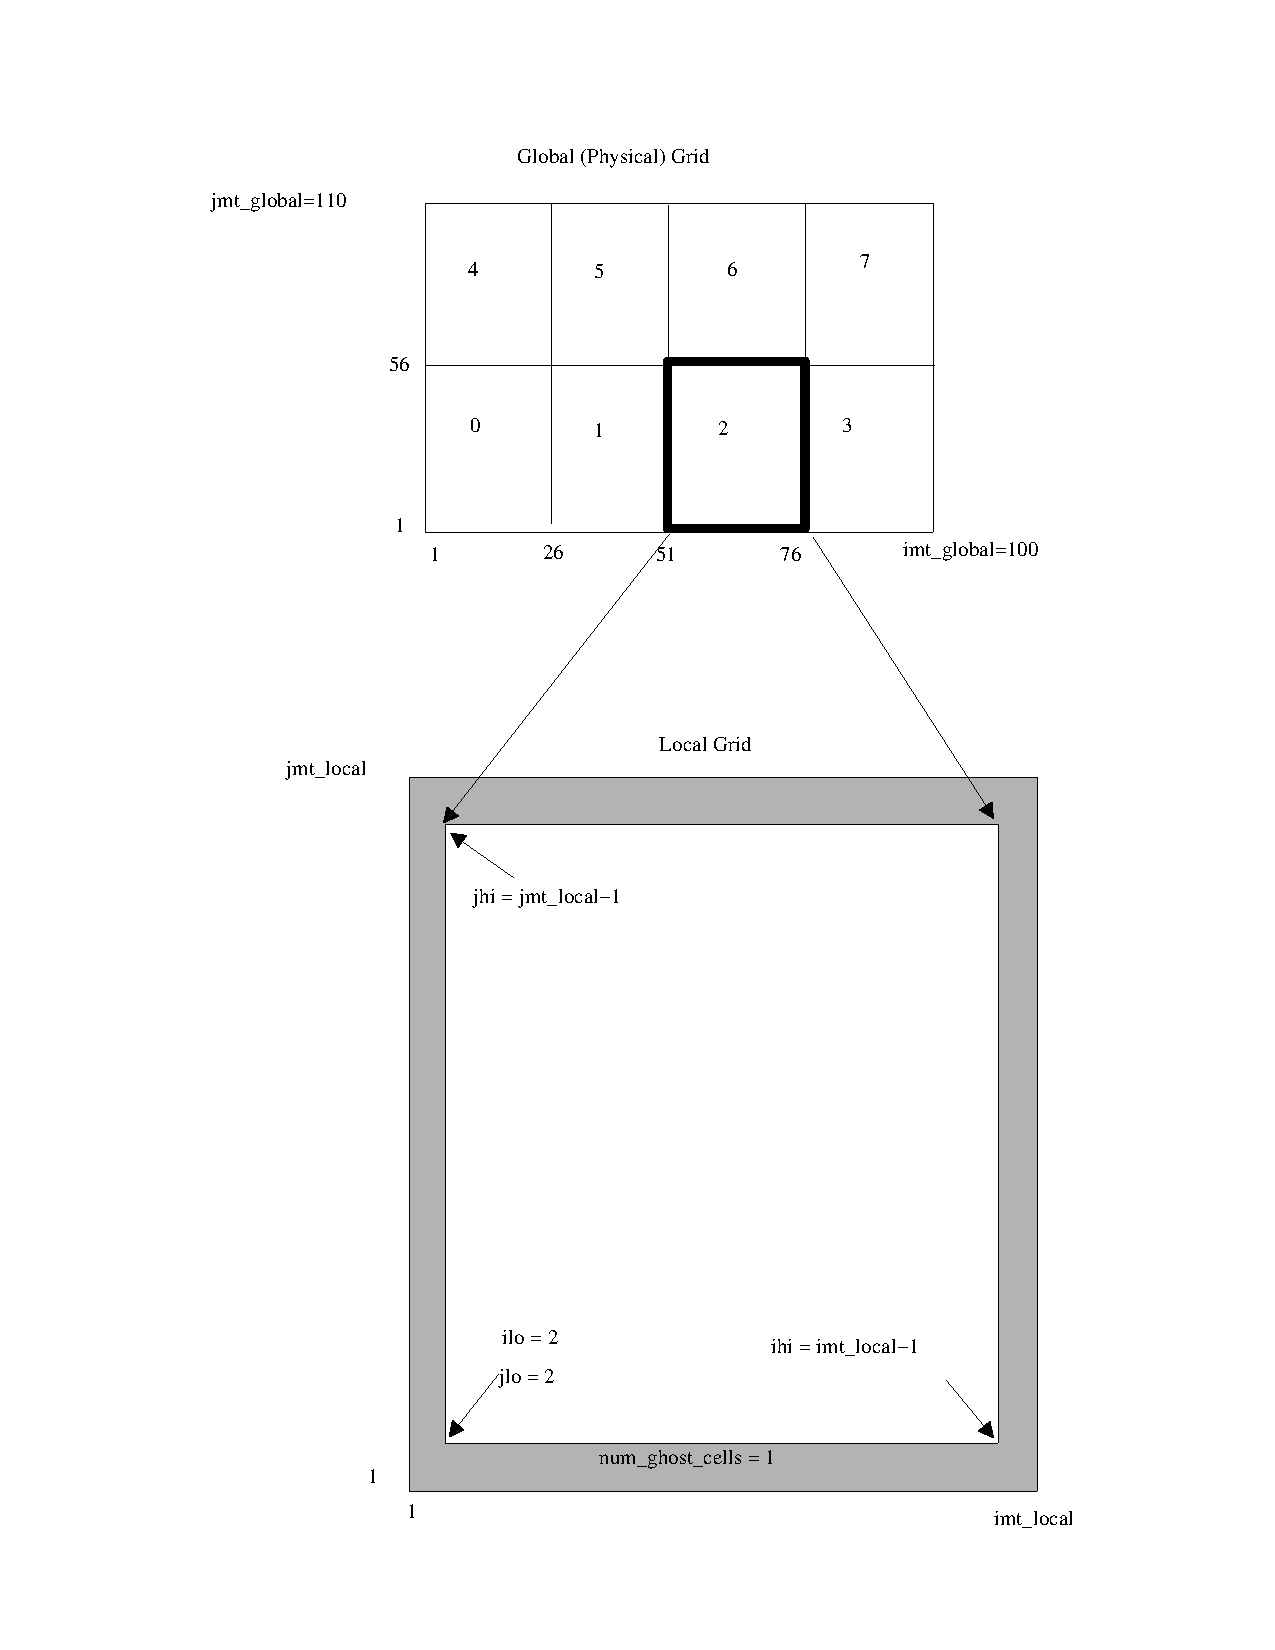
\includegraphics[height=8in]{ice_grid_schematic}  
  \caption{An example of the gx3 (imt\_global=100, jmt\_global=116) grid
           with the following decomposition: 4 processors in the x direction,
           2 in the y direction.  Grey shading represents ghost cells that
           are filled in by a call to {\it bound} with redundant data from
           neighboring processes.}
\label{fig:ice_grid_schematic}
\end{figure}
 

%\section {Making Code Modifications} 
%=======================================================================
% CVS: $Id: ice_making_mods.tex 5 2005-12-12 17:41:05Z mvr $
% CVS: $Source$
% CVS: $Name$
%=======================================================================

\section {Making Code Modifications} 

The source code for CSIM is located in {\bf ccsm3/models/ice/csim4/src/source}.

\begin{Ventry}{NOTE:}
\item[NOTE]
      The source code in this directory, and any code that has been checked out of
      the CVS repository should be treated as frozen code.  It is recommended that
      the permissions on these files be changed to read only.  To modify a module
      in CSIM, whether running coupled or uncoupled, first copy that module to a 
      separate directory.  If running CSIM coupled, this directory is near the 
      top of the CCSM directory tree and is called 
      {\bf ccsm3/scripts/\$YOUR\_CASE/SourceMods/src.csim}.  If running CSIM uncoupled,
      make a directory under the active ice component called \\
      {\bf models/ice/csim4/src/src.ice}.
      Make the modifications to the copied file.  The scripts are set up so that
      these directories are the last in the filepath, so the modified files are the last
      copied to the executable directory.
      This is a highly recommended programming practice, keeping your modifications
      separate from the original code.
\end{Ventry}

\subsection {Write Statements and Error Messages}

Adding write statements to source code that is using multiple processors can
produce unexpected results if not done correctly.  Generally, diagnostic write statements
should be done only by the controlling processor, called the {\tt master\_task}.  The
task number for the master processor is always zero and is set in {\it setup\_mpi}. The
master task is the only processor that can write to the log file.  If other tasks are
allowed to write to the log file, output from the master task will most likely be overwritten.
Write statements should be surrounded by an 'if' block:

\begin{verbatim}
if (my_task == master_task) then
  write (nu_diag,*) 'istep1:',istep1
endif
\end{verbatim}

Without the 'if' statement, all processors will write out the information.
Output from other processors will be written to the standard output file.

\subsubsection*{Finding Error Messages}

Errors that cause the ice model to stop do not always occur in the master task
subdomain, so there may not be information about the error in the log file.
When the model stops, look for error messages in the log files, standard output,
standard error, fort.*, and core files.  Since multiple processors are writing to
the standard output file, the error that caused the model to stop is not always right
at the bottom of the file.

\subsection {History Fields}

Adding a field to the history namelist is different than adding a field to
the history file.  If the field is already in the namelist, it can be added
or removed from the history file simply by modifying the namelist called
{\bf ice\_fields\_nml}. This is discussed in the CSIM User's Guide.

The fields that are available to the history file namelist are set in 
{\bf ice\_history.F}.  At the top of this module are instructions on
what to modify there, in the namelist in the ice setup script, and in
subroutines {\it init\_hist} and {\it ice\_write\_hist}.


\subsection {Restart Fields}

Fields that are necessary for an exact restart should be added to the
restart file.  These are binary files that are read by the ice model
for initial conditions for almost all types of runs.   There are
two subroutines in {\bf ice\_history.F} called {\it restartfile} and
{\it dumpfile} that read and write these files.  The actual reading of
the unformatted file is done by subroutine {\it ice\_read} in module
{\bf ice\_read\_write.F}.  New fields should be added to the end of the
restart file to allow backwards compatibility, i.e. older versions of
the model should be able to read the new restart file.  There is code in
{\it restartfile} that checks for the end of the file.  Currently, the
salt flux is the last field in the file.  If this field is present, it
is read in, if not, it is set to zero.  An exact restart test should be
done after modifying the restart file.  This test is automated in the
CSIM and CCSM scripts.  Adding more fields to the restart file should
only be done if required by physics changes.  It needs to be done
carefully, considering the need for backwards compatibility.


%\section{Code Management under CVS}
%=======================================================================
% CVS: $Id: ice_code_cvs.tex 5 2005-12-12 17:41:05Z mvr $
% CVS: $Source$
% CVS: $Name$
%=======================================================================

\section{Code Management under CVS}

CSIM uses {\bf \textsl{CVS}} for revision control.  CVS is a tool that documents the
history of source code changes and maintains this history on a source tree.  It documents
each change with a time stamp and the user name of the person who made it.  The
user making the changes adds some text describing the changes.  A tag is created,
which gives a label to the collection of revisions.

Tags on the {\bf \textsl{CVS main trunk}}, the main line of development for CSIM, are of the
form csim\#\_\#\_\#, where \# represents an integer.  
Modifications to the first number are for major model versions that usually coincide
with CCSM releases.  Increments are made to the middle number when model physics are
significantly modified or added.  These versions are typically not publically released.
Changes to the last number represent incremental changes to the model, such as bug fixes
or cosmetic changes.

Development work that is experimental or requires major code changes should be done
on a {\bf \textsl{CVS branch}}, a line of development separate from the main trunk. Branches
are used so that the changes do not appear on the main trunk until they
are thoroughly tested.  CVS branch names are of the form csim\#\_\#\_\#\_brnch\_desc
where the first three numbers denote the tag on the main trunk where the branch was
created.  The string of characters at the end of the tag name gives the purpose of the
branch. For example, csim4\_8\_16\_brnch\_bugfix was rooted at version csim4\_8\_16 on
the main trunk, and is a branch to make a bug fix.  Tags created along the branch should
have the form csim\#\_\#\_\#\_brnchT\_desc\#.  This is basically the branch name with a
'T' to differentiate the tag name from the branch name, and a number at the end to 
denote where along the branch the tag was made.


%\section{Coding Standard}
%=======================================================================
% CVS: $Id: ice_code_std.tex 5 2005-12-12 17:41:05Z mvr $
% CVS: $Source$
% CVS: $Name$
%=======================================================================

\section{Coding Standard}

The goal of a coding standard is to create source code that follows
a consistent style, giving the sea ice model a common look and better
readability.  For historical reasons, the current code does not
completely conform to all of the following standards.  Work is in 
progress to correct this. The coding standard will be enforced through
code reviews.

%============================================================================
\subsection{Style Guidelines}

\subsubsection*{General Guidelines}

\begin{itemize}

\item {\bf Fortran 90 Standard} CSIM uses the F90 standard.

\item {\bf Preprocessor} The C preprocessor is required as the macro
                         processor (cpp).  All tokens should be
                         uppercase to distinguish them from fortran code.
                         The use of ifdef constructs should be avoided
                         wherever possible.  The option should be set in
                         the namelist instead.

\item {\bf Fixed-Form Source} Fixed-form source will be used for readability.
       Columns 7 to 72 of a line may contain a Fortran statement, while columns
       1 to 6 are reserved for special purposes.  Blanks may be used freely
       anywhere.  Exclamation marks should be used to denote comments.
       A statement may include a maximum of 19 continuation lines. 

\item {\bf Bounds Checking} All code should be able to run when the following
      compiler options are set:
      \begin{itemize}
        \item Array bounds checking
        \item Automatic variables are initialized to NaN
        \item Floating point exception conditions: overflow, division by zero, and
              invalid operations 
      \end{itemize}

\end{itemize}

%---------------------------------------------------------------------------
\subsubsection*{Modules}

\begin{itemize}
  \item The use of modules is strongly encouraged since they provide global
        access to variables.
  \item Modules must have the same name as the file in which they reside,
        due to dependency rules used by "make" programs.        
        This implies that multiple modules are not allowed in a single file.
  \item Module names must begin with "ice\_".  This will provide unique
        module names when CCSM is released as a single executable version.
  \item Related subroutines and variables should be placed in
       a single module/file rather than keeping a single routine per file.
  \item The use of common blocks is discouraged.  Modules are a better
        way to provide access to declared entities via the "use" statement.
  \item If possible, access to variables should be limited through use of
        {\tt only} and {\tt private} clauses in the "use" statements.
\end{itemize}

%---------------------------------------------------------------------------
\subsubsection*{Subroutines}
\begin{itemize}
  \item {\bf \textsl{Inline}} any subroutine or function that is only called once, unless
        it contains a significant amount of physics.
  \item Minimize work arrays and other extraneous copies unless the array is
        used multiple times within the same subroutine.  Globally accessible
        work arrays are available in {\bf ice\_work.F}.
\end{itemize}
%---------------------------------------------------------------------------
\subsubsection*{Loops}

\begin{itemize}
  \item  Loops should be structured with the {\tt do}-{\tt enddo} construct as
         opposed to numbered loops.
  \item  Loops should be combined as much as possible for readability and
         performance.
  \item  Subroutine calls within loops over horizontal indices i and j should
         be avoided to produce a more vector-friendly code.
  \item  Short loops should be placed outside of longer loops to produce 
         vector-friendly code.  For example, loops over ice thickness categories
         should be placed outside of loops over horizontal indices {\it i}
         and {\it j}.
\end{itemize}

%---------------------------------------------------------------------------
\subsubsection*{Array Syntax}

\begin{itemize}
  \item Whole array expressions are encouraged for performance reasons.
        For example,
  \begin{verbatim}
                 do i = 1, imt
                   a(i) = b(i) + c(i)
                 enddo
  \end{verbatim}
  is more desirable than
  \begin{verbatim}
                 a = b + c
  \end{verbatim}
   
\end{itemize}

%---------------------------------------------------------------------------
\subsubsection*{Allocatable Arrays}
\begin{itemize}
  \item Allocatable arrays should be avoided for performance reasons.
\end{itemize}
%---------------------------------------------------------------------------

\subsubsection*{Variable Names}

\begin{itemize}
  \item {\bf State Variables} Primary state variables should use the following
         naming convention:
  \begin{itemize}
    \item {\tt aicen(i,j,n)} ice concentration for each ice category
    \item {\tt aice(i,j)} ice concentration aggregated over all ice categories
    \item {\tt ain(n)} ice concentration in a single column, for each ice category
  \end{itemize}

  Variables that are not state variables but are used in a similar manner should
  also follow this naming convention.  Note that {\tt ai} is not a good choice
  for a variable name.

  \item {\bf Descriptive Names} Variable names should be descriptive and long
        enough to be found, for example with the UNIX "grep" utility, without
        pages of extraneous material.  For example,
        {\tt eice} and {\tt esno} are preferable to {\tt ei} and {\tt es}.
 
  \item {\bf Variables with Similar Names} Variables with the same name, but
         with different numbers of arguments should not be used in different
         places.  For example, an array {\tt Ts(i,j)} in one subroutine should
         not be used as a local variable {\tt Ts} in another.  An exception
         to this would be the {\tt work} arrays, which should always be local.
\end{itemize}
%---------------------------------------------------------------------------

\subsubsection*{Variable Declarations}

\begin{itemize}
  \item  Variables should be declared in F90 format, using a double colon.
  \item  The F90 {\tt kind} type should be used for all variable declarations.
  \item  Continuation lines are encouraged for declarations of arrays that
         have similar kinds and dimensions.  For example:
  \begin{verbatim}
      real (kind=dbl_kind), dimension (imt_local,jmt_local) ::
     &   aice     ! concentration of ice
     &,  vice     ! volume per unit area of ice          (m)
     &,  vsno     ! volume per unit area of snow         (m)
  \end{verbatim}
  \item Variables should be declared one per line to allow a comment field
        after it, with a "!" character followed by the comment text.
  \item Variables of a similar type and function may be grouped together on
        a single line.  For example:
  \begin{verbatim}
     integer (kind=int_kind) :: nyrp,mdayp,weekp       ! previous year, day, week
  \end{verbatim}
\end{itemize}
%---------------------------------------------------------------------------

\subsubsection*{Code indentation}

\begin{itemize}
  \item Code within loops and if blocks will be indented three characters.
  \item Continuation lines of an assignment statement should begin to the
        right of the assignment operator.  For example, 
  \begin{verbatim}
   Fresh(i,j) = Fresh(i,j) + (vsn(nc)*Rside*rhos
  $                        +  vin(nc)*Rside*rhoi)/dt
  \end{verbatim}
  \item Continuation lines of a subroutine call should begin to the
        right of the "(" character.  For example, 
  \begin{verbatim}
   call comp_matrices  ( rowflg, hin, Hmean,
  $                      Gamm, HGamm, H2Gamm )
  \end{verbatim}
\end{itemize}
%---------------------------------------------------------------------------
\subsubsection*{Commenting of code}

\begin{itemize}
  \item  Comments enclosed in horizontal lines are "major":
  \begin{verbatim}
  !-----------------------------------------------------------------
  ! initializations
  !-----------------------------------------------------------------
  \end{verbatim}
  while those indented to match the following pertinent code are "minor":
  \begin{verbatim}
  ! compute aggregate ice state and open water area
  call aggregate
  \end{verbatim}

  \item Short comments can be included on the same line as the source code
        preceded by the "!" character.
  \item Comments on adjacent lines should be aligned, if possible.
\end{itemize}

%----------------------------------------------------------------------
\subsubsection*{Portability}
\begin{itemize}
  \item  The code will run on all platforms supported by CCSM.  See the CCSM
         User's Guide for the most recent list of supported machines and platforms.
  \item  Code should be developed using standard MPI (Message Passing Interface).
  \item  The code should run efficiently on cache-based and vector machines.
  \item  Standard F90 and MPI should be used so that the code is easily
         portable to other platforms.
\end{itemize}

%----------------------------------------------------------------------
\subsubsection*{Incomplete and dead code}
\begin{itemize}
  \item Incomplete code should be indicated by comments that include "TBD".
  \item Variables that are declared but not used should be removed.
  \item Code that is commented out should either be removed or contain
        comments as to why it is still there.
\end{itemize}

%----------------------------------------------------------------------

\subsubsection*{Miscellaneous}
\begin{itemize}
\item Tabs should not be used for spacing; they create a large inconvenience
      when editing.
\item Code will be written in lower case.  This differentiates Fortran code
      from C preprocessor tokens, since the convention has been established
      that these are upper case.
\item Use of the relational operators $<$, $>$, $<$=, $>$=, ==, and /= are preferred
      to {\tt .lt., .gt., .le., .eq.,} and {\tt .ne.} for purposes of readability.
\item The {\tt stop} command should be avoided when exiting the code after an
      error. Instead, the subroutine {\it abort\_ice} should be called.
\end{itemize}

%=====================================================================
\subsection{Content Guidelines}
%=====================================================================


\begin{itemize}
  \item {\bf Sign Conventions}  Enthalpy is defined as negative; fluxes
        are positive downward.

  \item {\bf Implicit None}  All modules will include an {\tt implicit none}
        statement, immediately following the {\tt use} statements.  This
        implies that all variables must be explicitly typed.

  \item {\bf Prologues}  Each module, subroutine and function will include
        a prologue for use with the ProTeX auto-documentation script
        (http://dao.gsfc.nasa.gov/software/protex).  This will be used
        to make a code reference document.
 
  \item {\bf I/O Error Conditions} I/O statements which need to check an
        error condition, i.e. namelist read statements, should use the 
        {\tt iostat = <integer variable>} construct instead of {\tt end} and
        {\tt err}.

  \item {\bf Intent} All dummy arguments should include the {\tt INTENT}
        clause in their declaration.

  \item {\bf Conditionals} Conditionals based on $<$ 0. or $>$ 0. should be avoided.

  \item {\bf Physical Constants} Values of physical constants should not be 
        hardwired into the executable portion of a code.  Constants should be
        defined in a single module as named, full-precision parameters.  
        
  \item All units should be in MKS; CGS conversions should be avoided.  
        Diagnostics and other fields that do not affect the model integration
        may be in other units.
\end{itemize}

%----------------------------------------------------------------------


%\section{Integration}
%=======================================================================
% CVS: $Id: ice_integrate.tex 5 2005-12-12 17:41:05Z mvr $
% CVS: $Source$
% CVS: $Name$
%=======================================================================

\section{Software Integration Procedure}

This section outlines the steps for testing and integrating newly developed
code into the existing sea ice model.  This procedure has been designed to
ensure that new code meets CCSM and CSIM requirements and improves the climate
simulation and/or the model performance.  All substantial code changes
must go through the Polar Climate Working Group ({\bf \textsl{PCWG}}) review process.
Substantial refers to all physics changes and any software engineering
changes that result in major changes to code organization and/or efficiency.
This generally does not include cosmetic changes to the code.

It may not be possible or necessary for a developer to carry out all of the steps
described in this section. For most development, it will be necessary to 
contact the liaison or a co-chair of the Polar Climate Working Group. This
information is on the PCWG web page: \\

\begin{htmlonly}
\htmladdnormallink{\tt http://www.ccsm.ucar.edu/working_groups/Polar/}
                      {http://www.ccsm.ucar.edu/working_groups/Polar/}. \\
\end{htmlonly}
\begin{latexonly}
  {\tt http://www.ccsm.ucar.edu/working\_groups/Polar/}. \\
\end{latexonly}

The PCWG review process will usually involve the following steps:

\begin{enumerate}
  \item Modeler develops improved code.  This can include modification
        of a few lines, improving a parameterization, or providing a
        new physics module.
  \item Modeler tests changes within CCSM framework.  See sections 
        \ref{control_run} and \ref{testing_mods}.
  \item Outcome of tests is posted on PCWG web site and modeler provides
        explanation to PCWG members.
  \item PCWG members review results (and code if desired).
  \item PCWG decide whether to recommend adoption of change to CCSM Code
        Review Board.
\end{enumerate}

\subsection{Making a Control Run}
\label{control_run}

Before new code is put into CSIM, a control run using the latest tagged
version of CCSM may need to be done to document the effects of the new
code on model performance and the simulated climate.  If newly
developed code is being put into a tagged version of CCSM, output from a
standard control run may already be available, in which case, this
set of steps can be skipped.  If output from a control run is not available,
here are the steps to create it:

\begin{enumerate}

  \item  Get a tagged version of CCSM via one of the following options:
    \begin{enumerate}
      \item  At {\bf \textsl{NCAR}}:
        \begin{enumerate}
          \item Check it out from CVS: {\tt cvs co -r ccsm\_tag\_name} 
          \item Copy it from {\tt /fs/cgd/csm/collections}
        \end{enumerate}
      \item  Off site:
        \begin{enumerate}
          \item Download it from http://www.ccsm.ucar.edu/models/ccsm3
          \item Contact the PCWG liaison or a co-chair for a copy.
        \end{enumerate}
    \end{enumerate}
  If you have questions regarding the appropriate CCSM tag name to use,
  contact a PCWG co-chair or the liaison.

  \item  See the CCSM User's Guide on how to set up the scripts for the 
         {\bf \textsl{M component set}} (latm, dlnd, docn, csim (mixed layer
         ocean mode), cpl).

  \item  Modify the latm source code and setup script to use your favorite
         forcing.  The PCWG can provide reasonable input datasets if needed.

  \item  Do a 10-15 year simulation to get a control run case, saving output
         in a permanent disk location.

  \item  Document performance by saving the timing information at the bottom of
         a log file, and put plots of output on web if necessary.  A graphics
         package is available for plotting output.

\end{enumerate}

\subsection{Testing Climate and Performance of Modified Code}
\label{testing_mods}

For purposes of adding new code to the existing model, a tagged version
of CCSM should be used, the more recent the better.  The latest version 
of CCSM will usually contain the latest version of CSIM. It is
a good idea to check if this is the case.  These are the steps for
integrating newly developed code into the existing sea ice model and testing:

\begin{enumerate}

  \item  Make modifications to the source code using one of the following options:
    \begin{enumerate}
      \item  Using CVS:
        \begin{enumerate}
          \item  Create a development branch from a CSIM tag on the main trunk, ideally
                 the CSIM tag used in the control run.
        \end{enumerate}
      \item  Not using CVS:
        \begin{enumerate}
          \item Copy modules to be modified from the source code directory to \\
                {\tt ccsm3/scripts/\$CASE/SourceMods/src.csim}, and make modifications
                in this directory.
        \end{enumerate}
    \end{enumerate}

  \item  Compile, run for 5 days with minimum debugging turned on: array
         bounds check, Nan initialization, floating point trap.

  \item  Check that code still meets any requirements that may have been
         affected by the new code.  The minimum tests are exact restart
         and conservation.  If developed code involves any namelist variables,
         all options for those variables must be tested.  Any tests
         available in the new code should be exercised.

  \item  Test on all supported platforms.  Compilation and a 5 day run are the
         minimum.

  \item  Do a 1 year run, check results against control run.

  \item  Continue run out to 10-15 years, saving output in a permanent disk location.
         This may be used as the next control run.

  \item  Document performance, compare with control run and put difference plots on web.

  \item  If results are satisfactory (approved by PCWG), code may be inspected
         and/or reviewed. Development branch will be merged with the main trunk
         and tagged.

  \item  Model documentation (User's Guide, Code Reference and Scientific Description)
         must be updated.

\end{enumerate}

Currently, there is no formal CCSM Requirements document, and the CSIM Requirements
document is still in the draft stage.  There is a somewhat complete list
of tests for CSIM, but an automated test suite is still under development.
All developers are strongly encouraged to read the CSIM Requirements Document
and all of the Developer's Guide (this document).

\subsubsection*{Minimum Requirements}

It is difficult to define all tests that are suitable for all code changes,
and a user may not have access to all supported platforms.  This section gives
a list of basic requirements for the ice model, to provide guidance for testing.
A more complete list of requirements is in the CSIM Requirements document
(under development).  As noted in section \ref{testing_mods},
any changes in climate or model performance due to the code modifications
must be documented.

\begin{description}

  \item [Minimum CCSM Requirements] Compiles, runs, and restarts exactly with
                        at least one configuration, preferably the 
                        {\bf \textsl{M component set}} (latm, dlnd, docn, csim in mixed
                        layer ocean mode, cpl) or the
                        {\bf \textsl{B component set}} (cam, clm, pop, csim, cpl).
              Runs on at least one standard CCSM grid (gx1v3 or gx3v5).
             Runs on all CCSM supported platforms available to the modeler.

  \item [Conservation] checking water, salt and energy budgets in the log file.
        Any conservation errors or CFL violations that occurred in the 10-15 year
        climate year run should be documented.

  \item [Exact Restart] This test is automated in the CSIM and CCSM scripts.
                       It does a 10 day startup run and a 5 day continuation
                       run that begins at day 5 of the startup run. Output from
                       days 5-10 of both runs are compared and must match bit-for-bit.

  \item [Debug Test] This test is also automated in the CSIM and CCSM scripts.

  \item[Input Data Files] If any new or modified input data files are necessary to
                          run the modified code, they must be provided with the code.
\end{description}


%\input{notes_for_guide}

%\section{Glossary}
\section{Glossary}

% USAGE NOTE:
%
% The first use of a term in the text of a document can be 
% linked to the corresponding glossary item using the item label.
% 
% For example,
%
% Original document text: code must include item1
%
% Linked to glossary:     code must include \htmlref{item1}{glos:item1}
%
% The link will appear in the html version of the document.
% The print version of the document will appear unchanged.

\begin{description}

\item [B component set] The shorthand name for the combination of all
                        active components of CCSM:  ocean, atmosphere,
                        land, and ice exchanging information via a coupler.

\item [CCSM] The Community Climate System Model is a fully-coupled,
             global climate model that provides state-of-the-art computer
             simulations of the Earth's past, present, and future climate
             states.

\item [CICE] The Los Alamos sea ice model

\item [CSIM] The CCSM Community Sea Ice Model 

\item [CSIM4] Version 4 of the CCSM Community Sea Ice Model that
              was released in May 2002 with CCSM2.0.

\item [CSIM5] Version 5 of the CCSM Community Sea Ice Model that
              was released in June 2004 with CCSM3.0.

\item [CVS]  The Concurrent Versions System used to record the
             history of source code.

\item [CVS branch] A line of development separate from the main trunk.

\item [CVS main trunk] The main line of development
                        on the CVS source tree.

\item [inline] An optimization where the code of called routines
               is inserted into the calling code to eliminate the calling overhead.

\item [LANL] Los Alamos National Laboratory

\item [load balancing]  The distribution of processing and communications
                        activity between components to minimize the resources used and the
                        time spent waiting by any single component. 

\item [M component set] The shorthand name for the combination of 
                        data ocean, atmosphere, and land models,
                        csim with the mixed layer ocean, exchanging
                        information via a coupler.

\item [MPI] Message Passing Interface is the protocol for passing messages
                             between parallel processors.

\item [NCAR] National Center for Atmospheric Research, in Boulder, Colorado

\item [PCWG] The Polar Climate Working Group is a team of scientists
             who develop and improve the sea ice component of CCSM,
             and who use the ice model alone or fully coupled in
             CCSM for studies of polar climate.

\item [ProTeX]  A perl script  that allows for automatic generation of
                Latex compatible documentation of source code, without a
                considerable effort beyond the documentation of the code itself. 

\end{description}










\bibliographystyle{../UsersGuide/jas}
\bibliography{../UsersGuide/master_list}
\addcontentsline{toc}{section}{References}

\appendix 
\section {Calling Tree}
\label{calling_tree}

This section contains the primary calling tree for the coupled ice model. Calls
to MPI, netCDF, share code routines, subroutines or functions within the ice model
that do not include ice physics (i.e. global\_scatter, get\_sum, bound, etc.) are
not included.  Calls to the slab ocean mixed layer model within the ice model are
shown in square brackets.

%=======================================================================
% CVS: $Id: ice_calltree.tex 5 2005-12-12 17:41:05Z mvr $
% CVS: $Source$
% CVS: $Name$
%=======================================================================

{\scriptsize
\begin{verbatim}
ICEMODEL
|
+-SETUP_MPI-+-ICE_COUPLING_SETUP
+-SHR_MSG_CHDIR 
+-SHR_MSG_DIRIO 
+-INIT_CONSTANTS
+-INPUT_DATA
+-INIT_GRID
| +-POPGRID
| +-COLUMNGRID
| +-RECTGRID
| +-TLATLON
| +-MAKEMASK
+-INIT_REMAP
+-INIT_CALENDAR
+-INIT_HIST
+-INIT_EVP
+-INIT_FLUX-+-INIT_FLUX_ATM
|           +-INIT_FLUX_OCN
+-INIT_THERMO_VERTICAL
+-INIT_ITD
+-INIT_MECHRED--COMP_MATRICES
+-INIT_STATE-+-AGGREGATE
|            +-BOUND_AGGREGATE
+-RESTARTFILE-+-AGGREGATE
|             +-BOUND_AGGREGATE
+-ALBEDOS
+-CALENDAR
+-[INIT_OCEANMIXED_ICE]
+-INIT_CPL
+-INIT_DIAGS
+-ICE_WRITE_HIST-+-PRINCIPAL_STRESS
|                +-ICECDF - write IC to netCDF file
|-----------------------------------------------
| BEGIN TIMESTEP LOOP
|-----------------------------------------------
+-FROM_COUPLER
+-[SET_OCEANMIXED_ICE]
+-INIT_MASS_DIAGS
+-THERMO_VERTICAL
| +-INIT_FLUX_ATM
| +-INIT_DIAGNOSTICS
| +-FRZMLT_BOTTOM_LATERAL
|----------------------------
| Loop through categories
|----------------------------
| +-INIT_COUPLING_VARS
| +-ATMO_BOUNDARY_LAYER
| +-INIT_VERTICAL_PROFILE
| +-ADD_NEW_SNOW
| +-TEMPERATURE_CHANGES-+-CONDUCTIVITY
| |                     +-ABSORBED_SOLAR
| |                     +-SURFACE_FLUXES
| |                     +-TRIDIAG_SOLVER
| +-THICKNESS_CHANGES
| +-MERGE_FLUXES
| +-UPDATE_STATE_VTHERMO
|----------------------------
| End loop through categories
|----------------------------
+-SCALE_FLUXES
+-TO_COUPLER
+-[TIME_INTRPLT_OCEAN_FORCING-+-OCNHEAT-+-ATMO_BOUNDARY_LAYER]
+-THERMO_ITD-+-AGGREGATE
|            +-BOUND_AGGREGATE
|            +-INIT_FLUX_OCN
|            +-REDUCE_AREA
|            +-REBIN-+-SHIFT_ICE
|            +-ZAP_SMALL_AREAS-+-NORMALIZE_STATE-+-AGGREGATE
|            +-LINEAR_ITD-+-AGGREGATE_AREA
|            |            +-COLUMN_SUM
|            |            +-COLUMN_CONSERVATION_CHECK
|            |            +-SHIFT_ICE
|            |            +-FIT_LINE
|            +-ADD_NEW_ICE-+-COLUMN_SUM
|            |             +-COLUMN_CONSERVATION_CHECK
|            +-LATERAL_MELT
|            +-FREEBOARD
+-EVP-+-EVP_PREP
|     +-STRESS
|     +-STEPU
|     +-EVP_FINISH
+-TRANSPORT_REMAP-+-DEPARTURE_POINTS
|                 +-LOCATE_TRIANGLES
|                 +-TRIANGLE_COORDINATES
|                 +-MAKE_MASKS
|                 +-CONSERVED_SUMS
|                 +-CONSTRUCT_FIELDS--LIMITED_GRADIENT
|                 +-FLUX_INTEGRALS
|                 +-UPDATE_FIELDS
|                 +-GLOBAL_CONSERVATION
|                 +-LOAD_TRACERS
|                 +-LOCAL_MAX_MIN
|                 +-CHECK_MONOTONICITY
|                 +-UNLOAD_TRACERS
+-TRANSPORT_MPDATA-+-CHECK_STATE
|                  +-MPDATA
+-RIDGE-+-RIDGE_MATRICES--COMP_MATRICES
|       +-RIDGING_MODE
+-ZAP_SMALL_AREAS
+-REBIN
+-AGGREGATE
+-BOUND_AGGREGATE
+-ALBEDOS
+-SCALE_HIST_FLUXES
+-RUNTIME_DIAGS
+-ICE_WRITE_HIST-+-PRINCIPAL_STRESS
|                +-ICECDF
+-DUMPFILE
|-----------------------------------------------
| END TIMESTEP LOOP
|-----------------------------------------------
+-EXIT_COUPLER
\end{verbatim}
}


\section {ProTeX Generated Documentation}

This appendix contains the module and subroutine documentation generated by ProTeX.
This section is available at \\
http://www.ccsm.ucar.edu/models/ccsm3/csim/RefGuide/ice\_refdoc/index.html .

%\input ice_protex.tex  % 

\end{document}


